\chapter{Literature Review}
\pagestyle{default}
\thispagestyle{default}

In this chapter, a literature review is provided in project-related areas. To build the framework (X-Fed NeuroScan: Federated Learning with Explainable AI for Medical Image Classification), we need to get familiar with foundations of medical image analysis, deep learning-based classification techniques, and the challenges associated with handling sensitive clinical data. We also examine the principles and methodologies of Federated Learning (FL) as a privacy-preserving approach for multi-institutional model training, as well as Explainable AI (XAI) techniques that enhance model transparency and clinical trust. Additionally, this chapter reviews existing commercial medical imaging applications, related academic research, and publicly available datasets. Finally, we evaluate the tools, platforms, and frameworks that support the development of deep learning models, federated learning workflows, and explainable AI components.

The chapter is organized as follows:

\begin{itemize}
	\item Section 2.1: Medical image history and challenges, with subsections on bone fractures and chest diseases.
	\item Section 2.2: Explainable AI (XAI) in medical image detection.
	\item Section 2.3: Federated Learning (FL) in medical image detection.
	\item Section 2.4: Combined approaches integrating detection with XAI and FL.
	\item Section 2.5: Summary of related papers.
	\item Section 2.6: Similar commercial applications.
	\item Section 2.7: Summary of the chapter.
\end{itemize}

\section{Medical Image Diagnosis}

\textbf{Medical imaging} is the cornerstone of modern diagnosis, providing non-invasive visualization of the body’s interior using techniques like X-rays, Computed Tomography (CT), and Ultrasound. Due to the high volume and complexity of medical scans, interpretation is often time-consuming and subject to human variability. This process is increasingly enhanced by \textbf{Artificial Intelligence (AI)}, particularly \textbf{Computer Vision (CV)} and Deep Learning (DL) methods.

While traditional Deep Learning (DL) approaches have achieved high accuracy in radiological analysis for disease detection and bone fracture localization, their clinical deployment is significantly hindered. The primary issues stem from two critical needs: the strict requirement for \textbf{data privacy} and the \textbf{black-box nature} of AI decision-making. These barriers prevent the widespread, trustworthy adoption of powerful AI models in healthcare settings.

Consequently, the research focus has shifted toward specialized solutions: \textbf{Federated Learning (FL)}, a privacy-preserving paradigm, and \textbf{Explainable AI (XAI)}, a necessary component for model transparency. This work provides a systematic review of the state-of-the-art in these domains. It begins by examining advanced deep learning architectures, analyzing the role of FL in data collaboration, and reviewing XAI techniques.

We will first detail the related work in chest X-ray diagnosis and bone fracture detection. Subsequently, it will explore the use of XAI and FL specifically within these two application areas, identifying the gap that this research aims to bridge.

\subsection{Chest Diseases Detection}

The chest, encompassing the thoracic cavity, houses vital organs such as the lungs, heart, and major blood vessels, making it susceptible to various respiratory diseases that can be detected through imaging techniques like chest X-rays (CXR). CXR is a non-invasive, cost-effective diagnostic tool widely used for identifying abnormalities in lung tissue. We focus on four key categories for multiclassification: pneumonia, tuberculosis (TB), COVID-19, and normal (healthy) cases.

\begin{itemize} \itemsep 10pt
	\item \textbf{Pneumonia} is an inflammatory condition of the lung alveoli, often caused by bacterial, viral, or fungal infections, leading to fluid-filled sacs visible as opacities on CXR.
	\item \textbf{Tuberculosis} is a bacterial infection primarily caused by Mycobacterium tuberculosis, characterized by granulomas, cavities, or nodular infiltrates in the lungs, which can be chronic and contagious.
	\item \textbf{COVID-19}, caused by the SARS-CoV-2 virus, presents with ground-glass opacities, consolidations, and bilateral lung involvement on CXR, often progressing rapidly.
	\item \textbf{Normal cases} exhibit clear lung fields without pathological signs, serving as a baseline for comparison.
\end{itemize}
Accurate detection of these diseases via deep learning (DL) models on CXR images is crucial for timely intervention, especially in resource-limited settings \cite{ref8} \cite{ref9}.

\subsection{Target Diseases and Their Radiological Characteristics}

This study focuses on three major respiratory diseases that can be detected through chest X-ray imaging: pneumonia, COVID-19, and tuberculosis. These diseases represent significant public health concerns worldwide and are among the most commonly investigated conditions in computer-aided diagnostic systems. Although all three diseases affect the respiratory system, each exhibits distinct pathological characteristics and radiographic features that can assist clinicians in diagnosis. Understanding their symptoms and appearance in chest X-ray images is essential for accurate interpretation and effective disease detection.

\subsubsection*{Pneumonia}

Pneumonia is an inflammatory condition of the lungs that primarily affects the alveoli, the small air sacs responsible for gas exchange. The disease is commonly caused by bacterial, viral, or fungal infections, leading to the accumulation of fluid or pus within the affected lung tissue. Pneumonia remains one of the leading causes of respiratory-related morbidity and mortality, particularly among young children, elderly individuals, and immunocompromised patients.

Common symptoms of pneumonia include:

\begin{itemize}
	\item Persistent cough, often accompanied by mucus production.
	\item Fever and chills.
	\item Shortness of breath.
	\item Chest pain, especially during breathing or coughing.
	\item Fatigue and general weakness.
	\item Rapid breathing in severe cases.
\end{itemize}

In chest X-ray images, pneumonia typically appears as areas of increased opacity, commonly referred to as consolidations or infiltrates. These opacities occur due to the accumulation of inflammatory fluids within the alveoli, reducing the normal air content of the lungs. Depending on the severity and type of infection, the abnormalities may be localized to a single lobe (lobar pneumonia) or spread across multiple regions of the lungs. The affected areas generally appear whiter than healthy lung tissue, which normally appears dark due to the presence of air.

\subsubsection*{COVID-19}

Coronavirus Disease 2019 (COVID-19) is a highly contagious respiratory illness caused by the SARS-CoV-2 virus. Since its emergence, COVID-19 has posed substantial challenges to healthcare systems worldwide due to its rapid transmission and potentially severe respiratory complications.

The clinical presentation of COVID-19 varies considerably among patients, ranging from asymptomatic infections to severe respiratory failure. Common symptoms include:

\begin{itemize}
	\item Fever.
	\item Dry cough.
	\item Fatigue.
	\item Shortness of breath.
	\item Loss of taste or smell.
	\item Sore throat.
	\item Muscle and body aches.
	\item Headache.
\end{itemize}

Chest X-ray findings associated with COVID-19 often include bilateral lung abnormalities, particularly in the peripheral and lower lung regions. The disease commonly manifests as patchy or diffuse opacities that may affect both lungs simultaneously. As the infection progresses, these opacities may increase in size and density, resulting in widespread pulmonary involvement. Severe cases can demonstrate extensive bilateral infiltrates that significantly reduce the visibility of normal lung structures. Although chest X-rays are useful for evaluating disease progression, early-stage COVID-19 infections may not always produce clearly visible abnormalities.

\subsubsection*{Tuberculosis}

Tuberculosis (TB) is a chronic infectious disease caused by the bacterium \textit{Mycobacterium tuberculosis}. The disease primarily affects the lungs, although it can also spread to other organs. Tuberculosis remains a major global health concern, particularly in regions with limited healthcare resources.

The symptoms of pulmonary tuberculosis often develop gradually and may include:

\begin{itemize}
	\item Persistent cough lasting several weeks.
	\item Coughing up blood or blood-stained sputum.
	\item Chest pain.
	\item Fever.
	\item Night sweats.
	\item Unexplained weight loss.
	\item Fatigue and weakness.
	\item Loss of appetite.
\end{itemize}

Tuberculosis exhibits a wide range of radiographic appearances depending on the stage and severity of infection. In chest X-ray images, the disease frequently affects the upper lung regions and may appear as patchy infiltrates, nodular lesions, or areas of consolidation. Advanced cases can produce cavitary lesions, which are hollow spaces formed by tissue destruction within the lungs. Fibrosis and calcified granulomas may also be observed in chronic or healed infections. The diverse presentation of tuberculosis can sometimes complicate diagnosis, as certain imaging features overlap with those of other pulmonary diseases.

\subsubsection*{Comparative Radiological Characteristics}

Although pneumonia, COVID-19, and tuberculosis all affect the respiratory system and produce abnormalities in chest X-ray images, their radiographic patterns often differ. Pneumonia commonly presents as localized consolidations caused by fluid-filled alveoli, whereas COVID-19 typically produces bilateral and diffuse opacities that frequently involve the peripheral lung regions. Tuberculosis often demonstrates upper-lung involvement, nodular infiltrates, and cavitary lesions, particularly in advanced stages of the disease. Recognizing these characteristic imaging patterns is crucial for differentiating between conditions and supporting accurate clinical diagnosis.

\subsection{Related Work in Chest Diseases Multi-class Classification}
Interpreting Chest X-rays (CXRs) is vital for diagnosing various thoracic diseases like pneumonia and tuberculosis. Due to the subtlety of findings and high image volume, \textbf{Deep Learning (DL)} models have been widely adopted to automate diagnosis. These models, trained on large datasets, primarily focus on \textbf{multi classification} of different chest diseases. The following research examples showcase the success of various \textbf{Convolutional Neural Network (CNN)} architectures in achieving high accuracy in CXR analysis.

\begin{itemize} \itemsep 10pt
	\item The researchers Develop an automated Deep Neural Network (CNN) to classify Pneumonia, COVID-19, Tuberculosis, and No-findings from chest X-rays, addressing limitations in individual disease detection and small/biased datasets in prior studies.
	they Created a custom CNN architecture with 5 convolutional blocks (16-256 channels, ReLU activation, max-pooling), trained on split data (80\% training, 20\% testing). They Addressed heterogeneous data sources by preprocessing images (resizing to 300x300, denoising, normalization, filtering) to create a coherent dataset of 21,581 images from multiple Kaggle sources they achieve accuracy 98.72\% (using validation metrics) , Outperformed SOTA schemes like Venkataramana et al. (96.6\%) and Bhandari et al. (94.54\%), The study proved that a large diverse dataset is essential to achieve high multiclass accuracy and prevent overfitting, though class imbalance slightly reduced COVID-19 performance (96.27\% recall) \cite{ref10}.
	\item The researchers Develop a custom CNN model with soft attention to classify chest X-ray images into normal, COVID-19, pneumonia, and tuberculosis, while analyzing misclassifications through handcrafted features and statistical methods to improve clinical interpretability and diagnostic reliability. , Utilized transfer learning with pre-trained CNN models (VGG-19, ResNet-50, EfficientNet, DenseNet), trained on a balanced dataset split into training (70\%), validation (15\%), and testing (15\%) sets. They Preprocessed images via normalization, data augmentation (rotation, flipping, zooming), and resizing; applied SMOTE at the feature level to balance the originally imbalanced dataset from heterogeneous sources Best Modelis  ResNet-50 with 
	Accuracy:  97\% Compared to VGG-19 (95\%), DenseNet (91\%), EfficientNet (94\%) \cite{ref11}. 
	\item This study proposed a multi-level classification model using CNNs to differentiate COVID-19 from Tuberculosis (TB) and other Pneumonias based on CXR images. The primary challenge was addressing the severe data imbalance, specifically the scarcity of COVID-19 samples. The novelty involved combining data augmentation with the SMOTE technique to artificially balance the minority class. The system employed a two-stage process: first, classifying TB versus general Pneumonia, and second, sub-classifying the Pneumonia cases into COVID-19 and viral/bacterial types. This multi-level approach was designed to significantly reduce misdiagnosis between these similar lung diseases. The model achieved a high accuracy of 97.4\% for the TB/Pneumonia stage. The second stage achieved 88\% accuracy for bacterial/viral/COVID-19 classifications, demonstrating an overall 8–10\% improvement over existing methods \cite{ref12}.
	\item Additionally, a unified DL framework like CXR-MultiTaskNet used ResNet50 for joint disease localization and classification, incorporating thoracic diseases like pneumonia and TB, with an F1-score of 96.5\% through shared feature extraction \cite{ref13}.
	\item Another deep-learning pipeline classified chest X-ray images into normal, pneumonia, TB, and COVID-19 using a sequential CNN approach. Preprocessing steps such as grayscale conversion and normalization improved robustness, while transfer learning enhanced performance on limited data. VGG-16 achieved 95.9\%, DenseNet-161 reached 98.9\% for distinguishing COVID-19 from pneumonia, and ResNet-18 obtained 76\% for COVID-19 severity classification. The study demonstrates the effectiveness of multi-stage CNN models for automated COVID-19 screening from CXR images\cite{ref14}.
	\item A knowledge-distillation deep-learning model classified CXR images into COVID-19, pneumonia, TB, and normal using the RDD4 dataset. A deep CNN teacher network transferred its knowledge to a lightweight student model built in Keras/TensorFlow, preserving accuracy while reducing complexity. Data imbalance was addressed through augmentation. The distilled student model achieved 96.08\% accuracy, with high precision and recall, showing strong suitability for real-time, low-resource deployment\cite{ref15}.
	\item They develop a custom CNN model with soft attention to classify imbalanced chest X-ray images into normal, COVID-19, pneumonia, and tuberculosis, 
	the approach Designed COV-X-net19, a 16-layer CNN architecture (4 conv layers, 6 max-pooling, soft attention, dropout, dense with SoftMax), trained on split data (70\% training, 10\% validation, 20\% testing) with ablation studies for hyperparameter optimization (ReLU, Nadam optimizer, LR=0.001, batch=32) , the technique used preprocessed images via text removal (OCR+inpaint), morphological opening (3x3 kernel), CLAHE (ClipLimit=5.0, TileGridSize=3x3), histogram equalization. Best Model: COV-X-net19 with accuracy: 95.18\% Compared to 8 trans fer learning models (e.g., MobileNet at 82.96\%, VGG16 at 62.46\%), base CNN (89.96\%), and SOTA studies with similar multi-class setups (e.g., accuracies below 95\% in imbalanced scenarios) \cite{ref16}.
	\item A CNN-based system classified chest X-ray images into COVID-19, pneumonia, TB, and normal using over 21,000 images from three public datasets. The model used five convolutional blocks with preprocessing steps such as resizing, denoising, and normalization to handle heterogeneous sources. It achieved a high validation accuracy of 98.72\%, with strong per-class performance across all categories. The study shows that a carefully designed CNN can effectively support joint diagnosis of major chest diseases from CXR images \cite{ref17}.
	
\end{itemize}

\section{Explainable AI (XAI) in Medical Image Diagnosis}

Explainable AI (XAI) refers to techniques that make the decision-making process of AI models transparent and interpretable, addressing the "black-box" nature of DL models by providing insights into why a prediction was made. In this project, XAI is integrated using methods like Gradient-weighted Class Activation Mapping (GradCAM), which generates heatmaps highlighting regions in medical images (e.g., fracture lines in bone X-rays or opacities in CXR) that influenced the model's classification. This linkage enhances trust in diagnostics for both bone fractures and chest diseases, allowing clinicians to verify AI outputs against radiological features, reducing misdiagnosis risks, and facilitating model debugging.

\begin{figure}[htb]
	\centering
	\begin{minipage}{0.55\textwidth} % Adjust width as needed
		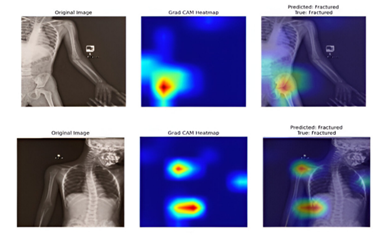
\includegraphics[width=\linewidth]{assets/bone_heatmap.png}
		\caption{Heatmap for bone}
		\label{fig:heatmap_bone}
	\end{minipage}
	\hfill % Adds horizontal space between minipages
	\begin{minipage}{0.40\textwidth} % Adjust width as needed
		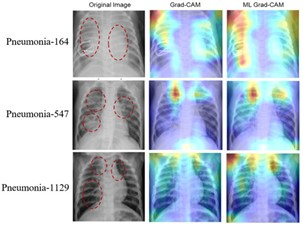
\includegraphics[width=\linewidth]{assets/pneumonia_heatmap.jpg}
		\caption{Heatmap for pneumonia detection}
		\label{fig:heatmap_pneumonia}
	\end{minipage}
\end{figure}

\subsubsection*{Related Papers on XAI For Bone Fracture Detection}
\begin{itemize} \itemsep 10pt
	\item Explainable AI has been increasingly integrated into medical imaging to ensure transparency  One study enhanced wrist fracture detection and classification by combining deep learning with XAI techniques, using saliency maps to highlight image regions that influenced predictions, thereby improving interpretability for clinicians. This work was presented in Enhancing Wrist Fracture Detection and Classification through Deep Learning and XAI (IEEE, 2024) \cite{ref18}.
	\item Another contribution focused on radiology, where machine learning models for bone fracture detection were augmented with XAI methods to visualize decision making processes. By providing interpretable outputs, the study bridged the gap between algorithmic accuracy and clinical usability. This was detailed in Enhancing Bone Fracture Detection in Radiology: A Machine Learning and Explainable AI Approach (IEEE, 2024) \cite{ref19}.
	\item Beyond fracture detection, interpretable machine learning has been applied to osteoporosis risk prediction. Comparative evaluations of predictive models were enriched with XAI analysis, allowing clinicians to understand how risk factors contributed to outcomes. This was reported in Interpretable Machine Learning for Osteoporosis Risk: A Comparative Evaluation of Predictive Models and XAI Analysis (IEEE, 2024) \cite{ref20}.
	\item Finally, advanced computational models have been proposed for predicting bone fracture healing and structural repair. XAI methods were employed to clarify how features influenced healing trajectories, supporting decision making in treatment planning. This was explored in XAI based Advanced Computational Models for Predictive Analysis of Bone Fracture and Structural Repair Healing Prediction (IEEE, 2024) \cite{ref21}.
	\item This study presents an Explainable AI system for humerus fracture detection utilizing deep learning models trained on 1,266 X-ray images from the MURA dataset. The researchers found that an ensemble of DenseNet architectures achieved a superior accuracy of 85\%, significantly outperforming standalone models like CNNs and VGGs. By integrating Saliency Maps and GRAD-CAM, the system visualizes specific fracture locations to ensure clinical interpretability and build trust with medical practitioners. This approach successfully combines high-performance automation with the necessary transparency for reliable orthopedic diagnosis \cite{ref22}.
	\item This study introduces a transparent AI framework for hand fracture detection using the YOLOv5m model trained on over 9,000 X-ray images. Optimized with specific preprocessing, the system achieved a superior 95.87\% accuracy, significantly outperforming architectures like Faster R-CNN in both speed and precision. The integration of Grad-CAM provides visual heatmaps with over 85\% localization accuracy, verifying that the model focuses on actual fracture lines rather than noise. This approach delivers a high-speed, interpretable diagnostic tool capable of enhancing clinical decision-making and trust \cite{ref23}. 
\end{itemize}

\subsubsection*{Related Papers on XAI For Chest Disease Multi-class Classification}
\begin{itemize} \itemsep 10pt
	\item This research introduces an Explainable AI (XAI) framework for the automatic detection, interpretation, and explanation of pulmonary diseases from chest radiographs (CXRs). The framework uses a transfer learning approach with a fine-tuned ResNet50 Convolutional Neural Network (CNN) trained on the COVID-CT and COVIDNet datasets. The Local Interpretable Model-agnostic Explanations (LIME) technique is employed to visually highlight the key regions in the CXR images that contribute most to the prediction. The developed system demonstrated strong performance, achieving high classification accuracy, reaching up to 97\% on the evaluated datasets. Validation confirmed that the model accurately focuses on clinically important features, thus assisting radiologists in early diagnosis and clinical decision-making\cite{ref24}.
	\item They develop XAI-TRANS, using inception-based transfer learning to classify CXR images for COVID-19, bacterial/viral pneumonia, and tuberculosis, addressing overlapping radiological features and black-box AI limitations by integrating improved U-Net segmentation and XAI tools the approach used is Utilized transfer learning with four pre-trained models (ResNet50, VGG19, VGG16, Inceptionv3), combined with an improved U-Net for lung segmentation to extract features, followed by XAI-TRANS for classification and explanation using Grad-CAM visualizations Technique Preprocessed images via resizing to 256*256 and normalization between 0 and 1fer learning models (e.g., MobileNet at 82.96\%, VGG16 at 62.46\%), base CNN (89.96\%), and SOTA studies with similar multi-class setups (e.g., accuracies below 95\% in imbalanced scenarios) the Best Model is XAI-TRANS (with and Grad-CAM) with accuracy: 97\% (overall classification accuracy) and 98\% precision, outperforming traditional DL methods by 4.75\% through XAI integration \cite{ref25}. 
	\item A survey reviewed over 200 papers on XAI in DL-based medical image analysis, emphasizing visual explanations for chest radiography to build clinician confidence\cite{ref26}.
	\item Additionally, an XAI-integrated DL framework for multiclass lung disease classification, targeting five classes: viral pneumonia, bacterial pneumonia, COVID-19, tuberculosis, and normal. It evaluates various DL architectures, including CNNs, hybrids, ensembles, transformers, and Big Transfer, with hyperparameter tuning and stratified 5-fold cross-validation to ensure robust performance. The Xception model, enhanced with transfer learning, emerges as the top performer, achieving 96.21\% accuracy by focusing on discriminative features in lung region\cite{ref27}.
	\item They built a lightweight CNN (5 convolutional layers) to classify chest X-rays into four classes: COVID-19, Pneumonia, TB, Normal. They applied Grad-CAM, LIME, and SHAP to generate visual explanations of model decisions, validating them with radiologists. The dataset was 7,132 public CXR images from three sources, with class imbalance handled by stratified batching. The model achieved a 10-fold cross-validation average test accuracy of 94.31\% ± 1.01\%, and they reported strong precision, recall, and F1\cite{ref28}.
\end{itemize}

\section{Federated Learning}

Federated Learning (FL) is a decentralized ML approach where models are trained collaboratively across multiple devices or institutions without sharing raw data, preserving privacy through local updates aggregated centrally. In medical imaging like bone X-rays and CXR classification, FL is used to train on distributed datasets from hospitals, mitigating data silos and complying with regulations like GDPR or HIPAA. It involves clients training on local data, sending model weights to a server for aggregation (e.g., via FedAvg), and is quickly implemented for real-time applications, reducing communication overhead while handling heterogeneous data.

\begin{figure}[htb]
	\centering
	\begin{minipage}{0.45\textwidth} % Adjust width as needed
		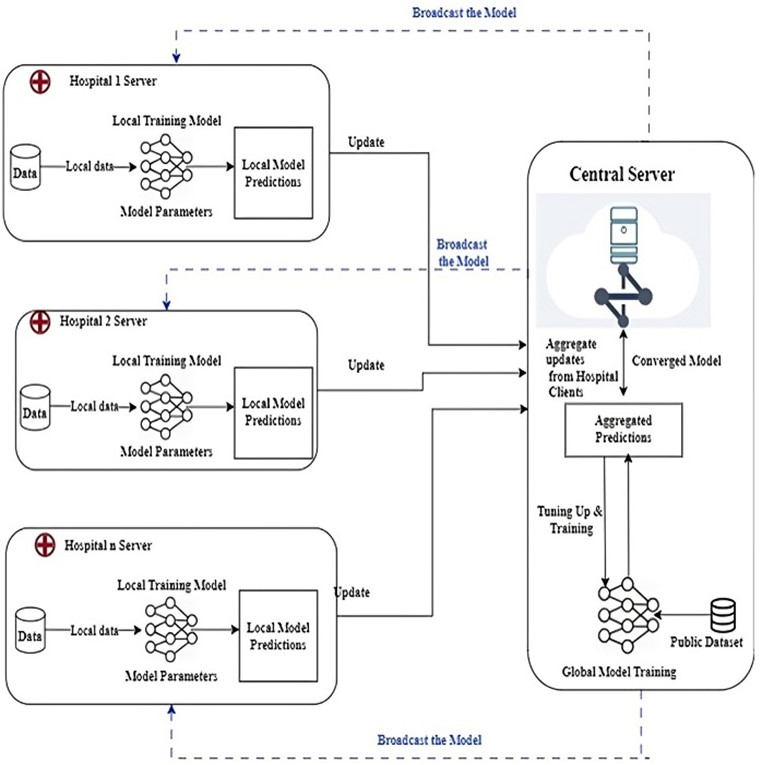
\includegraphics[width=\linewidth]{assets/federated1.jpg}
	\end{minipage}
	\hfill % Adds horizontal space between minipages
	\begin{minipage}{0.45\textwidth} % Adjust width as needed
		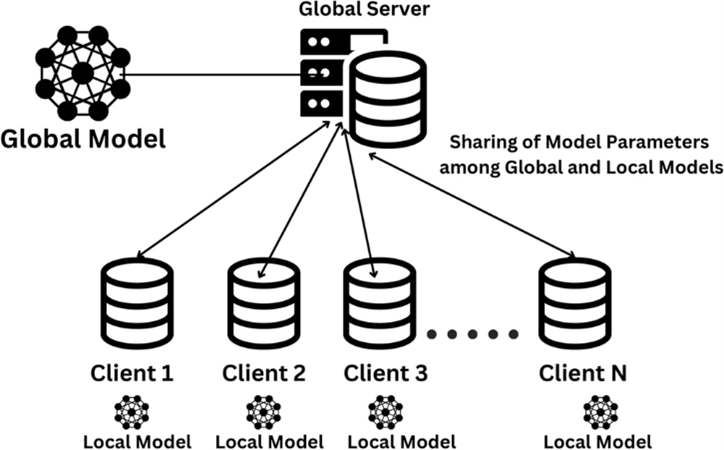
\includegraphics[width=\linewidth]{assets/federated2.png}
	\end{minipage}
	% Add more minipages for additional figures
	\caption{FL-Based efficient framework for smart healthcare sector}
	\label{fig:combined}
\end{figure}

\subsubsection{Related Papers on FL For Chest X-ray Disease Multi-class Classification}
\begin{itemize} \itemsep 10pt
	\item This study addresses the primary challenge in applying Federated Learning to chest X-ray analysis, which is the significant non-IID data distribution between adult and pediatric cohorts from different institutions. Analyzing over 400,000 radiographs, the research showed that conventional FL struggles to maintain consistent performance, particularly with the challenging pediatric dataset. The authors proposed enhancing FL by integrating general-purpose Self-Supervised Learning representations, using the DINOv2 model as a robust initialization.vThe new SSL-equipped framework proved highly effective, achieving an improvement exceeding 20\% in the AUC metric for pneumonia diagnosis in the difficult pediatric cases. This validates that readily available SSL models provide a practical and scalable solution for enabling FL in diverse healthcare settings while preserving data privacy\cite{ref33}.
	\item This study focuses on using federated learning (FL) for the accurate and privacy-preserving diagnosis of pediatric pneumonia via chest X-ray classification. Traditional machine learning approaches face significant challenges related to centralizing sensitive medical data, which risks patient privacy and security. FL addresses this by enabling collaborative model training across different institutions while ensuring the raw patient data remains local and secure. The researchers specifically tackled the common problem of data heterogeneity, which typically compromises classification accuracy in real-world clinical settings. They proposed an improved FL method utilizing "two-end control variables," modifying the loss function on the client side and adding momentum on the server. This novel approach successfully enhanced performance, achieving an average accuracy of 98\% and demonstrating an approximate 2\% improvement over existing federated learning algorithms. \cite{ref33}.
	\item Artificial Intelligence for lung disease detection is limited by major privacy concerns due to the need to centralize sensitive patient data (X-ray and CT scans). To overcome this, the paper proposes a decentralized Federated Transfer Learning (FTL) system, which enables effective collaborative model training without ever pooling raw data. This approach leverages federated learning's privacy features and the efficiency of transfer learning to train models on limited local datasets. The study evaluated four methods using the ResNet-50 model, confirming FTL as the most effective method for high accuracy. Specifically, the resulting accuracies were: Centralized (87.95\%), Transfer (88.04\%), Federated (87.55\%), and FTL (89.96\%) \cite{ref34}.
	\item A federated learning framework distinguished COVID 19 from four other chest diseases (lung cancer, TB, pneumothorax, pneumonia) plus normal using chest X rays from multiple hospitals. They used three pre trained models (DenseNet 169, VGG 16, VGG 19) and applied SMOTE to mitigate class imbalance. The aggregated system (using DenseNet 169) achieved 98.45\% accuracy, Grad CAM was used for model explainability, and their decision making client selection strategy reduced communication overhead significantly \cite{ref35}.
\end{itemize}

\section[Combined Approaches]{Combined Approaches: Medical Image Diagnosis with XAI and Federated Learning}

Integrating XAI and FL in medical image diagnosis combines privacy with interpretability, enabling collaborative training on bone X-rays and CXR while explaining predictions, with potential for broader medical domains. This section details key papers that merge these elements.

\subsection*{Related Papers on Combined Approaches for Chest Diseases Detection with XAI and Federated Learning}
\begin{itemize} \itemsep 10pt
	\item A Federated Learning Based Real Time Ensemble Model with Explainable AI Framework for an Efficient Diagnosis of Lung Diseases. It is FLEM-XAI, a privacy-preserving FL framework with XAI for real-time lung disease diagnosis from CXR, using FedAvg for decentralized training across hospitals without data sharing. It ensembles pre-trained models (InceptionV3, Conv2D, VGG16, ResNet-50) trained locally, aggregated centrally, and incorporates XAI via SHAP for feature importance and GradCAM for heatmaps highlighting affected lung areas. Results show ResNet-50 achieving 95.5\% overall accuracy (97.72\% COVID-19, 95.42\% pneumonia, 93.17\% TB), outperforming centralized models in bandwidth efficiency and maintaining convergence \cite{ref37}.
	\item This study introduces FLPneXAINet, a framework that securely predicts pneumonia from Chest X-ray (CXR) images by integrating Federated Learning (FL), Deep Learning (DL), and Explainable AI (XAI) to overcome data privacy issues. The method utilized an 8,402-image Kaggle dataset, which was augmented using a CycleGAN network, and then features were extracted via pre-trained DL models and four Ensemble DL (EDL) models. Feature optimization was performed using RFE, ANOVA, and RF to select the most relevant features, which were then classified by various machine learning models in an FL environment. The EDL network achieved the best results in the FL environment, with a high accuracy of 97.61\%, and was validated using XAI techniques (LIME and Grad-CAM). The full performance metrics were: F1 score 98.36\%, recall 98.13\%, and precision 98.59\%, offering a robust solution for healthcare professionals \cite{ref38}.
	\item A secure lung cancer prediction used mapreduce blockchain FL with XAI, ensuring interpretability in federated settings \cite{ref39}.
\end{itemize}

\section{Summary of Related Papers}
\renewcommand{\arraystretch}{1.2}
\begin{center}
	
	
	\begin{longtable}{|p{1cm}|p{1.5cm}|p{2cm}|p{1.8cm}|p{5cm}|p{1.2cm}|}
		\caption{Summary of related papers.} \\
		\hline
		\textbf{Focus Area} & \textbf{Sub-category} & \textbf{Model} & \textbf{Dataset} & \textbf{Result} & \textbf{Ref. Num.} \\ \hline % 
		Bones & General & Custom CNN and transfer learning & \textbf{FracAtlas} & The custom CNN achieved superior performance with 95.96\% accuracy, significantly outperforming the transfer learning models (EfficientNetB0, MobileNetV2, ResNet50) which only managed between 65\% and 67\% accuracy. & [1] \\ \hline
		
		Bones & General & YOLOv11 was developed and benchmarked against \textbf{Faster R-CNN} and SSD. & --- & YOLOv11 achieved superior performance with 96.8\% mAP and 95.14\% accuracy, significantly outperforming Faster R-CNN (87.5\% mAP) and SSD (82.9\% mAP) in both real-time fracture detection and localization. & [1] \\ \hline
		
		Bones & General & YOLOv11 was developed and benchmarked against Faster R-CNN and SSD. & --- & YOLOv11 achieved superior performance with 96.8\% mAP and 95.14\% accuracy, significantly outperforming Faster R-CNN (87.5\% mAP) and SSD (82.9\% mAP) in both real-time fracture detection and localization. & [1] \\ \hline
		
		Bones & General & EfficientNet-B6 & FracAtlas & The EfficientNet-B6 model achieved a 96.83\% testing accuracy & [3] \\
		\hline
		Bones & General & Custom CNN & ------ & The model achieved a classification accuracy of 92.44\% & [4] \\
		\hline
		Bones & General & SVM, k-NN, Naïve Bayes & -------- & Support Vector Machine (SVM) classifier achieved the highest accuracy, with a classification rate of 98\%. & [5] \\
		\hline
		Bones & General & Custom CNN & & Accuracy: 89.865\% (Approx. 90\%), Specificity: 89.90\% & [6] \\
		\hline
		Bones & General & Custom CNN & MURA dataset & Testing Accuracy: 99.79\% (at epoch 13). & [7] \\
		\hline
		Bones & XAI & MobileNetV3 style convolutional blocks with self-attention layers. & NEU Surface Defect Database, MVTec AD (Anomaly Detection), Severstal Steel Defect Dataset & proposed EdgeViT-Slim achieved 96.0\% accuracy, 0.953 F1 score, and 85 FPS on industrial defect datasets, outperforming baselines with far fewer parameters & [18] \\
		\hline
		Bones & XAI & ResNet-50, Faster R-CNN, and Mask R-CNN with Grad-CAM explainability & MURA & achieving 83\% classification accuracy (ResNet-50) & [19] \\
		\hline
		Bones & XAI & Random Forest, SVM, and KNN & MURA & Random Forest classifier achieved the best performance with 95\% accuracy, 93\% precision, and 0.96 F1-score, outperforming SVM (91\%) and KNN (88\%) & [20] \\
		\hline
		Bones & XAI & Logistic Regression, Random Forest, XGBoost, AdaBoost, LightGBM, and Gradient Boosting & custom multi-center clinical osteoporosis dataset (1,250 records) & ensemble model achieved the best performance with 90.82\% accuracy, 100\% precision, 81.63\% recall, and 89.99\% F1-score & [21] \\
		\hline
		Bones & XAI & (CNN, VGG, DenseNet) and found that Ensemble-2 (combining DenseNet121 and DenseNet169) & MURA dataset & The Ensemble-2 model achieved the highest accuracy of 85\% and an F1 score of 0.79. Additionally, the integration of Explainable AI (Grad-CAM and Saliency Maps) & [22] \\
		\hline
		Bones & XAI & YOLO, Faster R-CNN, & ------- & YOLOv5m (Best Performer) Achieved a Pointing Game Accuracy of $>85$\%, meaning Grad-CAM heatmaps consistently aligned with the ground truth fracture locations. & [23] \\
		\hline
		Bones & FL & DenseNet161 & & Federated Learning (FedAvg): The 5-node FedAvg model achieved the best performance with 91\% accuracy. Centralized Training: The centralized DenseNet161 model achieved 89.6\% accuracy. & [29] \\
		\hline
		Bone & FL & Local ML Models (Client-side), Federated Learning Frameworks (Server-side) & -- & Highest accuracy of 94.4\% (FL+VGG16 with augmentation) for binary classification. & [30] \\
		\hline
		Bones & FL & EfficientNet V2 (implemented within an Adaptive Federated Learning framework) & --- & federated methods lagged slightly behind the 96–98\% accuracy achieving near-centralized performance of up to 98.6\% using EfficientNetV2 & [31] \\
		\hline
		Bones & Combined & SemFedXAI (a framework combining Semantic Web technologies and Federated Learning & ------ & The SemFedXAI framework achieved the highest predictive accuracy at 85.3\%, outperforming standard Federated Learning (73.5\%) and other baselines. It also demonstrated superior explainability, scoring 0.85 in feature identification accuracy & [36] \\
		\hline
		Chest & General & Custom CNN & Kaggle \& IEEE & The model achieved 98.72\% overall accuracy across all classes. Recall per class: Pneumonia 99.66\%, No-findings 99.35\%, Tuberculosis 98.10\%, COVID-19 96.27\%. & [10] \\
		\hline
		Chest & General & & Kaggle & Accuracy: 97\% (using Resnet-50) VGG-19 (95\%), DenseNet (91\%), EfficientNet (94\%) & [11] \\
		\hline
		Chest & General & Custom CNN & Kaggle & TB vs Pneumonia classification: 97.4\% accuracy; COVID-19 vs viral/bacterial pneumonia vs (other pneumonia types) classification: 88.0\% accuracy & [12] \\
		\hline
		Chest & General & Custom CNN & VinDr-CXR & Classification Accuracy = 96.8\% (from micro-F1 $\approx$ 0.968) Localization Accuracy $\approx$ 85\% (IoU $\approx$ 0.851) & [13] \\
		\hline
		Chest & General & VGG16, DenseNet-161 and ResNet-18 & Custom clinical dataset collected and labeled & Normal/Pneumonia/TB/ COVID-19 classification (via VGG-16): 95.9\% . Normal/Pneumonia/COVID-19 classification (via DenseNet-161): 98.9\% . COVID-19 severity classification (via ResNet-18): 76.0\% . & [14] \\
		\hline
		Chest & General & Custom CNN & Kaggle & 97\% average accuracy (with precision $\approx$ 94\% and recall $\approx$ 97\%) for the full classification task. & [15] \\
		\hline
		Chest & General & Custom CNN and VGG-16 & Kaggle \& public dataset from Github & The COV-X-net19 achieves 95.18\% , MobileNet :  82.96\%, VGG16 : 62.46\% and  base CNN : 89.96\% . & [16] \\
		\hline
		Chest & General & DenseNet201, ResNet152V2 & IEEE & The model achieved superior performance with a test accuracy of 98.87\%, outperforming the individual base models (DenseNet201 and ResNet152V2) and demonstrating robust multi-class classification capabilities. & [17] \\
		\hline
		Chest & XAI & Explainable Framework based on DenseNet-201 & -- & The proposed explainable DenseNet-201 model achieved a high classification accuracy of 98.08\%, while also providing visual explanations (Grad-CAM) to build trust and interpretability for clinical diagnosis. & [24] \\
		\hline
		Chest & XAI & CNN and Vision Transformer & Kaggle & XAI-TRANS achieves accuracy: 97\% and 98\% precision & [25] \\
		\hline
		Chest & XAI & Review of various Deep Learning models and XAI techniques (e.g., Grad-CAM, LIME) & Survey of medical image analysis studies & & [26] \\
		\hline
		Chest & XAI & Custom CNN with Grad-CAM and LIME & -- & The proposed Custom CNN model achieved a high classification accuracy of 98.41\%, with XAI techniques successfully highlighting the critical image regions used for diagnosis, thereby improving model interpretability. & [27] \\
		\hline
		Chest & XAI & Ensemble of DenseNet201, InceptionResNetV2, Xception with Grad-CAM++ & Kaggle \& IEEE & The proposed deep learning ensemble achieved a superior average classification accuracy of 98.97\%, with XAI visualizations providing clinically plausible explanations for the model's decisions across all disease classes. & [28] \\
		\hline
		Chest & FL & Federated Learning (FedAvg) with a ResNet-based backbone and a novel age de-biasing loss function. & Multi-institutional chest X-ray datasets & The proposed de-biased FL model achieved an AUC of 89.7\%, outperforming the standard FL model (AUC of 86.2\%) and demonstrating significantly improved fairness and accuracy across different age groups. & [32] \\
		\hline
		Chest & FL & Federated Averaging (FedAvg) algorithm with a DenseNet-121 architecture as the core CNN model. & Chest X-ray images from multiple clients & The federated DenseNet-121 model achieved a test accuracy of 96.7\% and an F1-score of 95.8\%, matching the performance of a model trained on centralized data while preserving privacy. & [33] \\
		\hline
		Chest & FL & Federated Transfer Learning using a pre-trained ResNet-50 model, fine-tuned collaboratively across sites. & Collection from Kaggle & The federated transfer learning model achieved a classification accuracy of 96.3\% for detecting various lung diseases, significantly outperforming models trained on single, isolated datasets. & [34] \\
		\hline
		Chest & FL & A custom Federated Learning framework using a specialized Composite-DenseNet & -- & The DMFL\_Net framework achieved a high overall classification accuracy of 98.21\% and a precision of 98.14\%, demonstrating superior performance for multi-disease classification in a federated setting. & [35] \\
		\hline
		Chest & Combined & A Federated Learning-based Real-Time Ensemble Model combining multiple CNNs (VGG16, ResNet) with XAI techniques like Grad-CAM. & Kaggle & The FLEM-XAI ensemble model achieved accuracy of 99.4\% for multi-class lung disease classification. & [37] \\
		\hline
		Chest & Combined & A Federated Deep Learning framework using a custom CNN architecture integrated with XAI methods such as LIME and SHAP for model interpretation. & Chest X-ray images from distributed clients & The proposed FLPneXAINet framework achieved a high accuracy of 98.7\% in detecting pneumonia from chest X-rays & [38] \\
		\hline
		Chest & Combined & A Secure Framework using MapReduce, Blockchain-based Federated Learning, and XAI with a DenseNet-201. & Multi-source CT scan datasets & The secure federated learning model achieved an exceptional accuracy of 99.8\% for lung cancer prediction, leveraging blockchain for security and XAI for providing transparent, interpretable results. & [39] \\ \hline
	\end{longtable}
\end{center}

\section{Datasets Utilized in the Project}

\begin{table}[h]
	\centering
	\caption{Summary of Datasets Used in the Project}
	\label{tab:datasets}
	\renewcommand{\arraystretch}{1.3}
	\begin{tabular}{|p{3cm}|p{2cm}|p{7.5cm}|p{2.5cm}|}
		\hline
		\textbf{Dataset Name} & \textbf{Domain} & \textbf{Class Distribution / Description} & \textbf{Total Images} \\
		\hline
		FracAtlas & Bone &
		Fractured (1707), Hand (3487), Hardware (210), Hip (796), Leg (5293), Shoulder (796) &
		9,383 \\
		\hline
		COVID-19 \& Pneumonia \& Tuberculosis with Normal \& Non-X-ray &
		Chest &
		COVID-19 (\num{3616}), Normal (\num{5688}), Pneumonia (\num{4861}), Tuberculosis (\num{3453}) &
		\num{17618} \\
		\hline
		Chest X-ray Dataset for Lung Segmentation &
		Chest &
		Annotated chest X-ray images for lung segmentation tasks &
		\num{6106} images with corresponding \num{6106} masks \\
		\hline
		Random Images for Image Classification &
		General &
		Unlabeled random images used for general image classification experiments &
		\num{9958} \\
		\hline
		MURA &
		Bone &
		Elbow (1,912), Finger (2,110), Hand (2,185), Humerus (727), Forearm (1,010), Shoulder (3,015), Wrist (3,697) &
		40,561 images (14,656 studies) \\
		\hline
	\end{tabular}
\end{table}



\section{Similar Commercial Applications}

Several commercial applications leverage AI for medical image diagnosis, providing tools for clinicians to detect conditions like bone fractures and chest diseases. These applications often use DL models for classification but may lack advanced XAI or FL features for interpretability and privacy. Below, we discuss some notable examples.

\subsection{Aidoc (aiOS™)}
Aidoc is a leading clinical AI software company that utilizes its proprietary aiOS™ platform to deliver high-performance AI solutions for medical imaging interpretation and workflow optimization. The platform automatically analyzes medical scans, prioritizing critical findings like stroke, pulmonary embolism, and intracranial hemorrhage, and then notifies care teams in real-time. By integrating seamlessly with existing systems like EHR and PACS, Aidoc's solutions help radiologists streamline workflows, enhance diagnostic accuracy, and accelerate time-to-treatment for patients with acute conditions across radiology, cardiology, and neurovascular specialties.
\begin{figure*}[h]
	\centering
	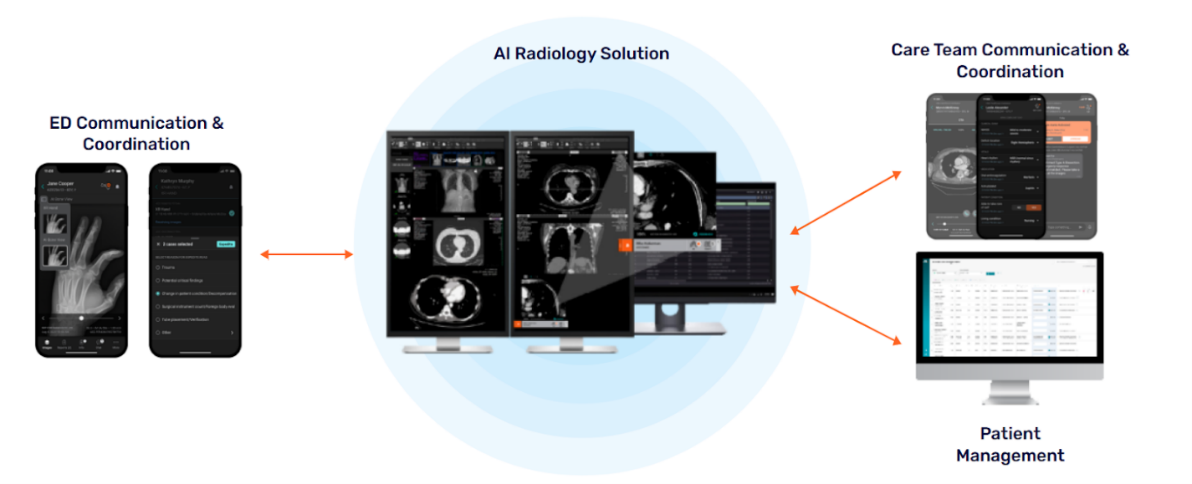
\includegraphics[width=0.5\linewidth]{assets/aidoc.png}
\end{figure*}

\subsection{Viz.ai (Viz.ai One®)}
Viz.ai is a leading AI-powered care coordination platform focused on transforming time-sensitive medical care by accelerating diagnosis and treatment decisions. The Viz.ai One® platform features multiple FDA-cleared AI algorithms that analyze imaging data, including CT scans and EKGs, to detect suspected diseases like stroke and pulmonary embolism. Crucially, it then uses real-time alerts and communication tools to instantly connect multidisciplinary care teams on mobile and desktop devices, ensuring the patient receives the necessary intervention as quickly as possible.
\begin{figure*}[h]
	\centering
	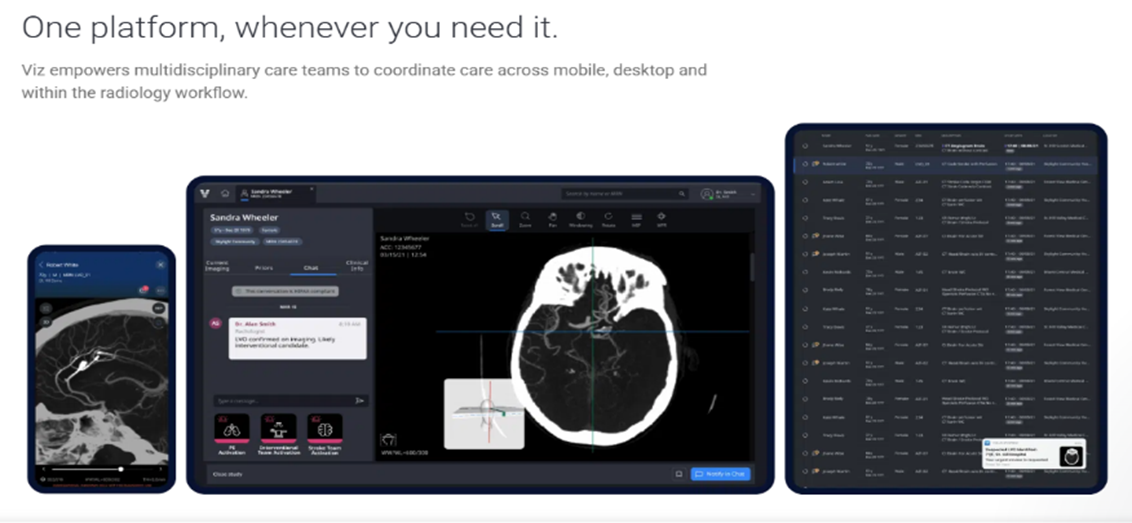
\includegraphics[width=0.5\linewidth]{assets/vizai.png}
\end{figure*}

\subsection{Qure.ai (qXR, qCT)}
Qure.ai specializes in developing deep learning algorithms for affordable and accessible diagnostics, with a strong presence in global health initiatives. Their core products, qXR (for chest X-rays) and qER/qCT (for head and lung CTs), use AI to detect and quantify abnormalities, including tuberculosis, lung nodules, and critical trauma findings. By analyzing scans with high accuracy in minutes, Qure.ai’s solutions assist radiologists in early disease detection, risk stratification, and provide essential diagnostic support, especially in areas with limited access to specialists.
\begin{figure*}[h]
	\centering
	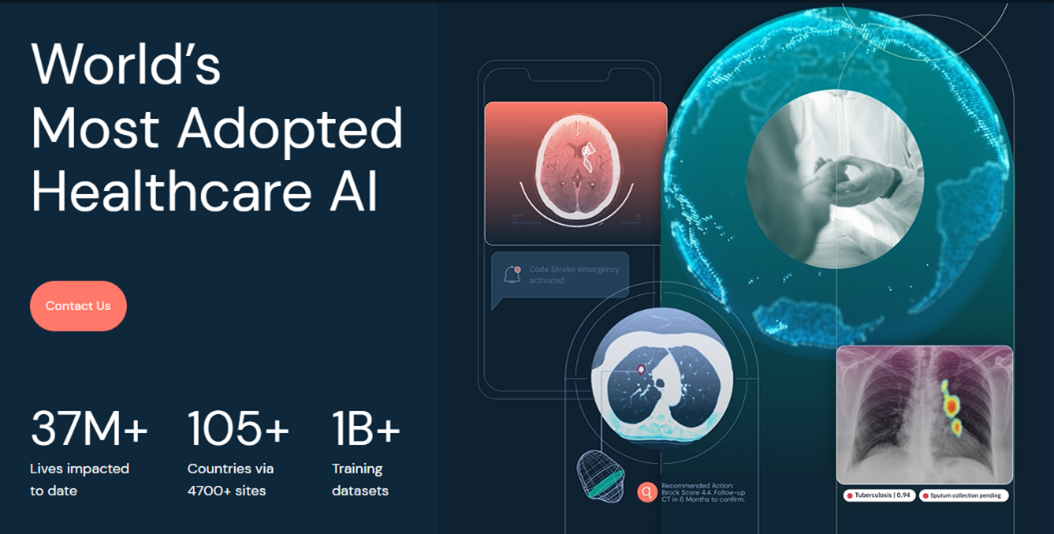
\includegraphics[width=0.5\linewidth]{assets/qure.png}
\end{figure*}

\subsection{Harrison.ai}
Harrison.ai, through its partnership with the I-MED Radiology Network 
(Annalise.ai), offers comprehensive, decision-supported AI tools designed to raise the standard of patient care and combat capacity limits. Their advanced AI solutions for Chest X-ray (CXR) and Non-contrast Head CT (CTB) are designed to detect a massive number of potential findings (often over 100) within seconds. By acting as a 'co-pilot' for clinicians, their AI solutions flag emergent and incidental findings, helping to reduce stress from chaotic worklists and significantly improving both diagnostic accuracy and efficiency.

\subsection{Lunit (Lunit INSIGHT, Lunit SCOPE)}
Lunit is a global leader in medical AI software with a singular mission to conquer cancer through cutting-edge technology. The company's solutions, including the Lunit INSIGHT suite for cancer screening (especially mammography and chest X-ray) and the Lunit SCOPE platform for precision oncology, transform complex clinical data into clear, actionable insights. By delivering highly accurate diagnostic results and extracting intelligence from tissue images to predict treatment response, Lunit empowers earlier detection and more precise treatment decisions across the entire cancer care continuum.

\section{Summary}

In this chapter, we presented the background on bone fractures and chest diseases as initial focus areas for medical image diagnosis, emphasizing multiclassification. We discussed similar commercial applications, reviewed related works on detection using DL for each domain, explainable AI techniques like GradCAM for interpretability (with potential image insertions for heatmaps), federated learning for privacy-preserving training, and combined approaches integrating these elements. We also evaluated tools for development. These insights form the foundation for our extensible project's development, highlighting gaps in interpretability and data privacy that our system aims to address for bone fracture detection, chest disease detection, and future expansions. \newpage